\begin{figure*}
 \centering
  \begin{subfigure}[b]{0.3\textwidth}
      \centering
      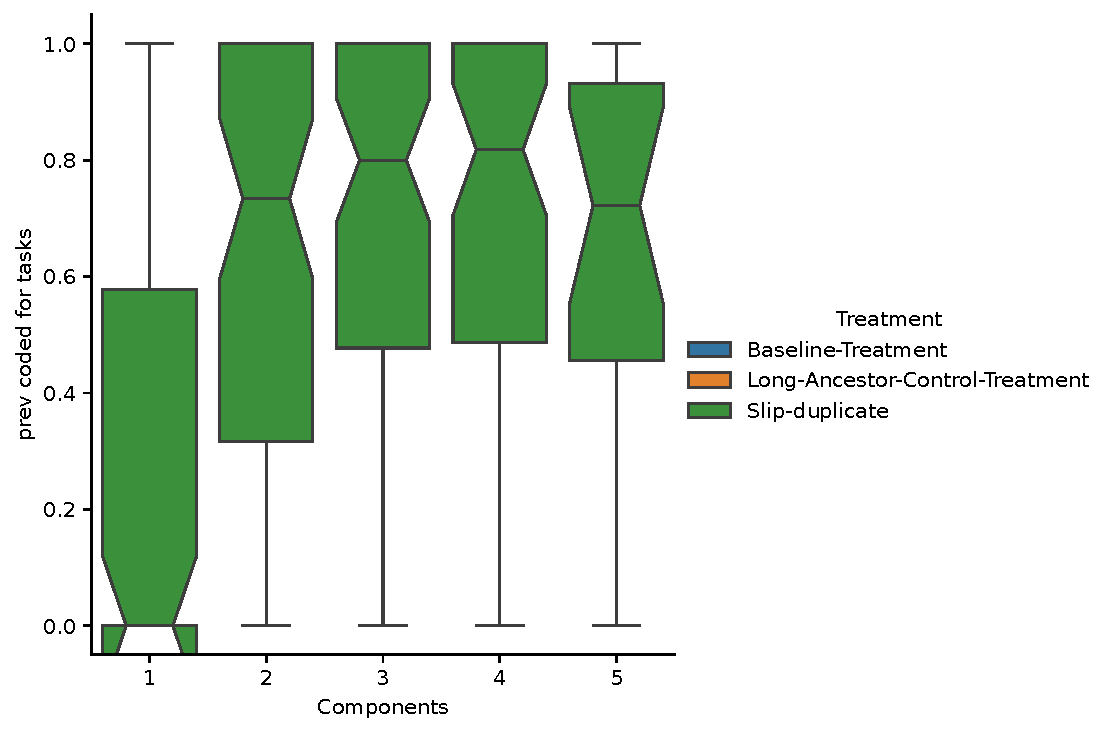
\includegraphics[width=\textwidth]{binder/binder/teeplots/hue=treatment+kind=box+viz=catplot+x=components+y=prev-coded-for-tasks+ext=}
      \caption{Previous Coded for Tasks, number sites}
      \label{fig:hard-task-gain-numsites-coded}
  \end{subfigure}
  \hfill
  \begin{subfigure}[b]{0.3\textwidth}
      \centering
      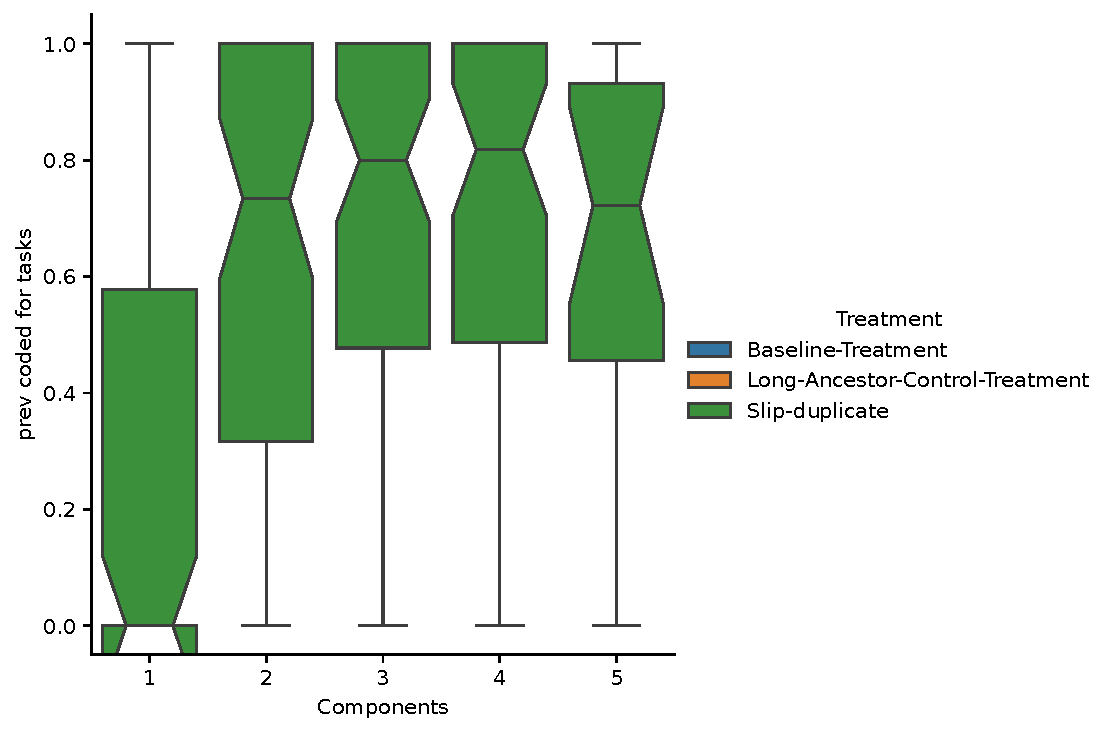
\includegraphics[width=\textwidth]{binder/binder/teeplots/hue=treatment+kind=box+viz=catplot+x=components+y=prev-coded-for-tasks+ext=}
      \caption{Previous Coded for Tasks, fraction new coding sites}
      \label{fig:hard-task-gain-fracsites-coded}
  \end{subfigure}
  \hfill
  \begin{subfigure}[b]{0.3\textwidth}
      \centering
      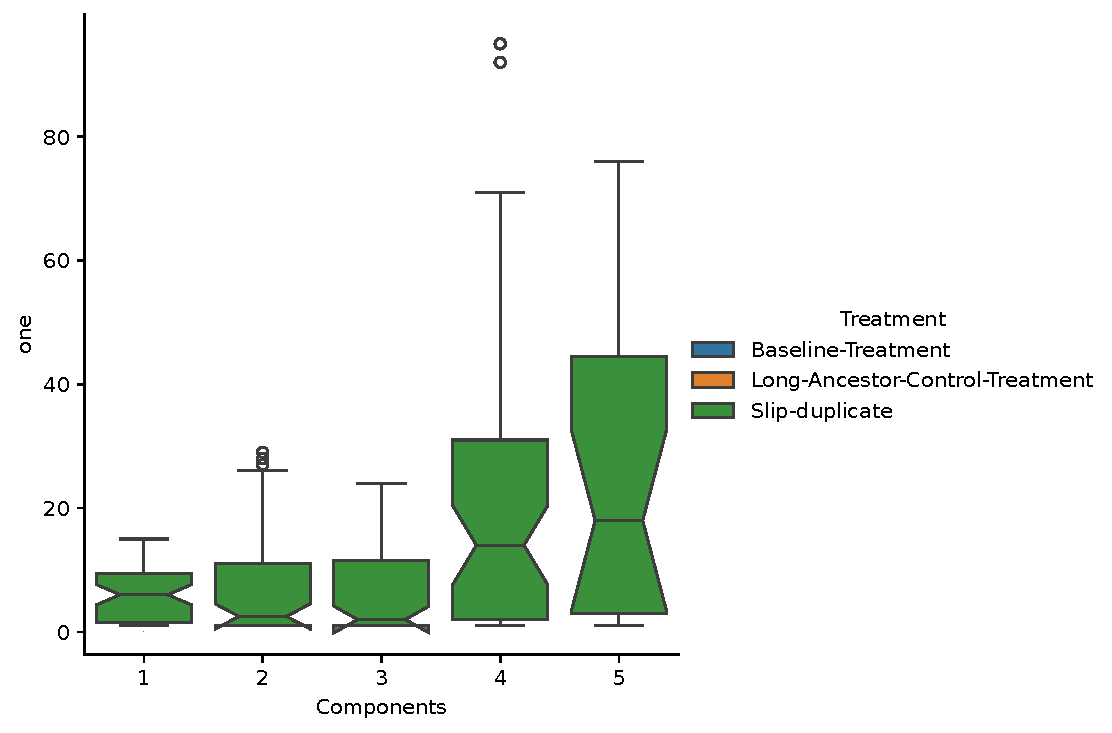
\includegraphics[width=\textwidth]{binder/binder/teeplots/hue=treatment+kind=box+viz=catplot+x=components+y=one+ext=}
      \caption{Number of new coding sites}
      \label{fig:hard-task-gain-numsites}
  \end{subfigure}
  \caption{
  \textbf{More complex tasks re-use more coding sites and involve larger number of coding sites.}
  \footnotesize
  TODO
  }
  \label{fig:hard-task-gain}
\end{figure*}
